\chapter*{General Introduction}\markboth{GENERAL INTRODUCTION}{}
\addcontentsline{toc}{chapter}{General Introduction}

"A knowledge economy is one in which knowledge assets are deliberately accorded more importance than capital and labor assets, and where the quantity and sophistication of the knowledge pervading economic and societal activities reaches very high levels" \cite{world2007building}.

The concept of a Knowledge Based Economy (KBE) has evolved and been debated among economists and policy makers, with different definitions and interpretations of what constitutes a knowledge economy and how to measure its progress and performance \citep{powell2004knowledge}. The fundamental principles of a KBE is the generation and dissemination of knowledge. Science plays a central role in this context and drives technological advancements as well as contributes significantly to both economic development and growth. Science help us understand the natural world, improve our quality of life and address societal issues. Science can help policy makers understand potential risks and hazards, such as natural disasters, pandemics, and emerging technologies. This enables them to create strategies and regulations to minimize risks or promote initiatives that are beneficial to society. 
Knowledge creation is the process of generating new knowledge, ideas, and insights that advance our understanding of the world. It involves the discovery of new information, the synthesis of existing information, and the development of new ways of thinking about problems and phenomena. One theory of knowledge creation in an organisational setting was developed by \cite{nonaka2006organizational}. The generation of new knowledge occurs through interactions between explicit and tacit knowledge via a process known as the socialization, externalization, combination, and internalization (SECI) spiral. Meaning that in order to understand how knowledge is created we need to look at the actors, the interaction between them but also the environment in which they are. Understanding the structure and dynamics of the scientific system is crucial for both fostering the growth of the KBE and addressing pressing challenges of our time, including climate change, poverty, and, as seen recently, global pandemics.

This thesis contributes to this endeavor and is organized in 3 chapters. \textbf{Chapter I} focuses on the scientific collaboration network's structure and resilience following an exogenous shock, namely the Covid-19 pandemic. \textbf{Chapter II}  breaks down the creativity aspect of scientific publications and look at how the profile of researchers affects novelty and impact, the pillars of creativity. Finally, \textbf{Chapter III} investigates the intersectoral mobility of AI researchers and the potential impact on their research.

In recent decades, there have been significant changes in the way research is conducted and how the scientific network is structured. The changes have been characterized by increased international mobility and collaboration among researchers, a decrease in solo authorship, and a rise in intersectoral mobility and collaboration \citep{geuna2015global}. The rise of International collaboration has been observed in multiple papers. There is an increasing trend of number of authors and international collaboration across country \citep{adams2012rise}. This result is corroborated in \cite{wagner2017growth} observing a growth of 120\% of Scientific international collaboration between 1990 and 2013. This is partly explained by the increase of countries participating in research (i.e more actors more possibility of collaboration). This increase is accompanied by a drop of the share of paper solo authored which seems to affect less younger researcher \cite{kuld2018rise}. While the accessibility to scientific knowledge is growing, team size is growing and agents increasingly specialize their competences to navigate into this growing knowledge landscape as it is too vast and complex for any individual agent to master it (\cite{boudreau2016looking}). Using OpenAlex, a fully open-source library designed to represent the global research system, containing over 240 million research documents \cite{priem2022openalex}, Figure \ref{fig:1} shows that these two trend continues to be observed recently.

\begin{figure}[H]
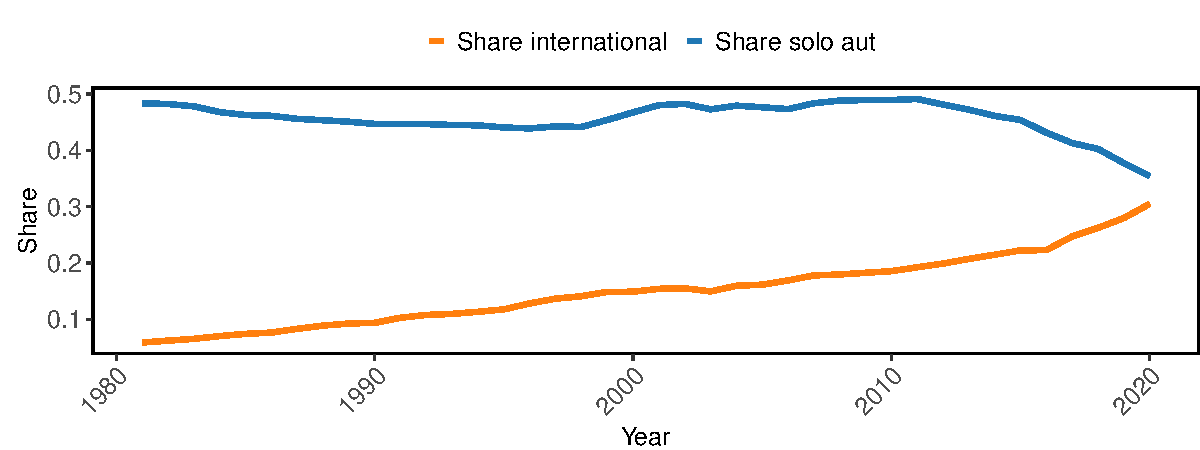
\includegraphics[width=0.9\textwidth]{0_Introduction/figures/Fig1.pdf} %
\caption{Evolution of the share of solo authorship and International collaboration in OpenAlex}
\label{fig:1} 
\end{figure}

In this context it is crucial to understand how the scientific collaboration structure emerges and how it evolves to answer urgent problematic. Multiple dimensions contribute to increasing the likelihood of a collaboration occurring between two authors. \cite{boschma2005proximity} distinguish 5 proximity dimensions that influences the possibility of co-authorship: Cognitive, Geographical, Institutional, Organizational and Social proximity. Cognitive Proximity refers to the similarity or compatibility of researchers' knowledge, expertise, and research interests. When researchers have similar cognitive backgrounds or work in related fields, it becomes easier to communicate and collaborate effectively. Geographical Proximity relates to the physical distance between researchers. When researchers are located in close proximity, such as working in the same institution or region, it facilitates face-to-face interactions, frequent meetings, and easier coordination for collaborative projects. Institutional Proximity could be better understood as the national context in which scientist evolves (i.e the "societal macro level"). Each country has their agenda, law and budget which then influences grant and the creation of collaboration. Organizational Proximity focuses on the affiliation context of researchers. Collaboration becomes more likely when researchers belong to the same or closely aligned organisation, as they share resources, facilities and research networks. Social Proximity relates to the social relationships and networks among researchers. Collaboration is facilitated when researchers have established social connections, such as shared professional networks, common collaborators, friendships, or mentor-mentee relationships, as trust and familiarity are already present. Although this taxonomy was meant for micro-level analysis they can also be useful to understand macro-level collaboration.

Scientific collaboration between countries is influenced by a number of factors. According to \cite{dosso2023towards}, region-specific factors play a significant role in shaping scientific collaboration between African countries. The study found that shared ethnic language, membership in the African and Malagasy Council for Higher Education (CAMES), and the presence of a common European partner as a third partner in co-publication were important factors in scientific collaboration. In addition to other determinants of scientific collaboration between countries include geographical distance, colonial heritage, and common language. However, these factors are shown to be decreasing in importance. This suggests that as scientific research becomes more globalized, other factors such as shared research interests and complementary expertise become more important.
Another important factor in scientific collaboration between countries is the presence of international networks and organizations that facilitate collaboration. For example, scientists from eight full member countries are working together within the SESAME community, as described by UNESCO\footnote{\url{https://www.unesco.org/en/scientific-research-cooperation-why-collaborate-science-benefits-and-examples}}. This organization provides a platform for scientists to collaborate and share expertise, despite political tensions between some of the member countries.
In addition to regional organizations, there are also global organizations that promote scientific collaboration, such as the International Science Council and the World Academy of Sciences. These organizations provide funding and support for international research projects and facilitate collaboration between scientists from different countries.
The level of scientific collaboration between countries can also be influenced by national policies and funding priorities. For example, \cite{hu2020mapping} reports that Greece, Portugal, Germany, and the Netherlands have ranked themselves among the highly collaborative countries recently, while Romania, Turkey, Sweden, Denmark, Ireland, England, and Scotland have all slipped down at least five spots. This suggests that changes in national policies and funding priorities can have a significant impact on scientific collaboration between countries. 

In order to comprehend the dynamics and structure of scientific collaboration, network theory is frequently employed. Researchers have utilized this approach to identify several noteworthy characteristics that define the system. One such characteristic is the emergence of a community structure within the network, which is often attributed to the triadic closure phenomenon \footnote{Recent studies have challenged this explanation \cite{kim2017over}}. This phenomenon, characterized by the tendency for individuals to form connections with others who share mutual connections, suggests that if person A collaborates with person B and person B collaborates with person C, there is a higher likelihood that person A will also collaborate with person C. Additionally, this community structure can manifest as a core-periphery structure, as demonstrated in previous research \cite{wedell2022center}. The consolidation of this core-periphery structure is further reinforced by the preferential attachment mechanism. This mechanism posits that newcomers to the network are more inclined to initially connect with the most reputable individuals. As a result, the scientific system ends up as a robust and resilient structure \cite{wagner2017growth}.

All of the above is proof that the scientific collaboration between countries is influenced by a complex set of factors. Yet the literature is still scarce on the dynamics of the scientific system after an exogenous shock. Covid-19 raised the question on how well the scientific system adapts to new urgent shock at the global scale. The goal of \textbf{Chapter I} was to gain insights on this phenomenon and answer two problematic. How did the structure of the coronavirus research evolve after the Covid-19 and how does the structure of global health sciences relate to the scientific response to the pandemic? We found a close coupling of national and international positioning in Coronavirus related
research (CRR). CRR capacity accumulated before the pandemic has been influential for national CRR output and international CRR collaboration at the beginning of the pandemic. Broader health science capacity became the dominant factor after. Global CRR during the pandemic rapidly converges towards the global order of
broader health science capacity but the mirroring is not perfect. This results shows that for a world wide shock the way that science organizes itself is by using the already existing channel. But is the existing channels of the global health science system efficient ? To answer that we need to understand how to measure research.

Paul Otlet initially defined bibliometrics in 1934 \citep{otlet1990traite}, and it was later reintroduced by \cite{pritchard1969statistical} in their paper titled "Statistical Bibliography or Bibliometrics?". The primary objective of bibliometrics was to prevent a "flood" of knowledge and facilitate its efficient utilization by enabling librarians to select relevant items for their collections \citep{sugimoto2018measuring}. In 1955, Garfield, a chemist and documentalist, proposed the establishment of a citation index. This led to the formation of the Institute for Scientific Information in 1960 by Garfield, which subsequently developed the Science Citation Index (SCI). The SCI was first launched in 1963 making it easier to locate and reference specific publications. It also calculates citation metrics, such as the number of times an article has been cited by other articles, which can be used to evaluate the impact and significance of scientific research. Since then, there has been an exponential growth in the number of scientific documents, as well as the proliferation of various channels (such as preprints and blog posts) and databases containing metadata associated with papers (such as Knowledge Graphs, Web of Science, Scite, and Crossref). Furthermore, alternative metrics (Altmetric) were developed using web data (Twitter likes/share being the most famous example). These developments have underscored the significance of managing the available pool of knowledge. Researchers and institutions focused on the impact and citation metrics aspect of publications. Grant evaluation, career opportunities are mainly driven by the h-index of authors. In parallel originality is not enough supported by research. If combination of topics in a grant proposal is too far from the knowledge domain of the grant Principal Investigator (PI) then it is less likely to win the grant. Meaning that to be part of the funding process you need to conform with the prevailing norms or conventions in your field. Yet novelty is crucial in science. First of, originality in science helps to promote a diverse range of ideas and perspectives. This diversity is essential for scientific progress, as it allows researchers to explore new avenues and challenge established paradigms. If originality is lacking, the field may stagnate, and the body of knowledge will not grow \citep{flexner2017usefulness,arnott2020co}. Second highly novel paper is more likely to be a breakthrough paper than more conventional \citep{wang2017bias,shibayama2021measuring}. Yet the factors which increases the likelihood of a highly novel research paper to be a breakthrough is still unclear.

\textbf{The second chapter} of the thesis is dedicated to exploring the creativity of the Health Science System. We specifically used the bipartite classification of creativity, which encompasses two key elements: novelty and impact\cite{runco2012standard}. We explore the relationship between cognitive diversity in scientific teams and their capacity to both foster innovative ideas and attain scientific recognition. An author-level metric based on semantic representation of researchers' past publications is proposed to measure cognitive diversity at both individual and team levels. We can think of our indicator as a measure of \textit{potential novelty}, i.e., opportunities for new knowledge recombination available through the diversity of backgrounds in the team and the capacity of individuals to bridge the gap between other team members. In comparison, combinatorial novelty indicators would capture the \textit{realized novelty}, i.e., the output of the research conducted by this team in terms of pieces of knowledge used. Finally, Faculty Opinion labelling and other external validation methods can describe the \textit{perceived novelty}, i.e., the peers' perception of this study. Seen from this perspective, we investigate whether \textit{potential} novelty contributes to \textit{realized} and \textit{perceived} novelty and its scientific recognition, measured with metrics of disruptiveness \citep{wu2019large,bornmann1911disruption,bu2019multi}. Using 1.8M articles from the 2000-2005\footnote{Restricting our sample to early 2000 allow us to avoid the potential biais of long term citation caused by ``sleeping beauties'' \citep{lin2021novelty}} PubMed Knowledge Graph (PKG), we analyze the impact of cognitive diversity on novelty, as measured by combinatorial novelty indicators but also peer labelling on Faculty Opinion. The findings reveal an inverse U-shaped relationship between cognitive diversity and average exploratory profiles within teams with combinatorial novelty and citation impact. It is demonstrated that the presence of highly exploratory individuals is beneficial for generating distant knowledge combinations, but only when balanced by a significant proportion of highly exploitative individuals. Moreover, teams with a high share of exploitative profiles consolidate science, while those with a high share of exploratory profiles disrupt it, particularly when associated with exploitative researchers. These results emphasize the significance of team composition in scientific creativity, indicating that a combination of exploratory and exploitative individuals leads to the most disruptive and distant knowledge combinations. Our findings emphasize the critical role of the cognitive dimensions in creativity, as it significantly influences originality and success. We show that cognitive diversity always seems beneficial to combine more distant knowledge. In contrast, the within-team average exploratory profile follows an inverse U-shaped relation with combinatorial novelty (i.e. there is a turning point where it is no longer beneficial). The same relation can be found when examining the impact in terms of citations. However, our study highlights the strong connection between the cognitive dimension and the nature of these citations. More specifically, teams with more \textit{exploitative} profiles tend to consolidate science, while those with more \textit{exploratory} individuals disrupt it when associated with \textit{exploitative} ones. 



The first two chapters focused on health science and with no sectoral distinction. Although the international mobility of researchers has been extensively studied, the determinant of scientists inter-sectoral mobility and its impact is still understudied and not well understood \cite{geuna2015global}. Universities play a critical role in knowledge creation, and their missions reflect this importance. The first two missions of universities are Teaching and Research. Universities are responsible for educating the next generation of scholars, professionals, and leaders. This involves providing high-quality instruction in a wide range of fields. On the other hand Universities are also responsible for conducting cutting-edge research that advances our understanding of the world and addresses some of the most pressing issues facing society \citep{secundo2017intellectual}. This involves pursuing new ideas and discoveries, testing hypotheses, and developing new technologies and innovations. In recent decades, changes in the national and international context have led to a transformation in the way universities and economic actors, such as companies, collaborate and the roles they play in society. The purpose of this transformation is to establish a connection between universities and society, which is commonly referred to as Universities' Third Mission (TM) \citep{zomer2011rise,secundo2017intellectual,compagnucci2020third}. The TM is generally concerned with knowledge transfer or knowledge exchange, which involves diffusing the knowledge generated by universities to society and contributing to the economic, social, and cultural development of the surrounding community. One of the channels of this TM is the link between academia and industry which can be decomposed in different collaboration type including the transition of a researcher from Academia to industry \cite{ankrah2015universities}. The increasing participation of Industry in fundamental research aswell as the growing intersectoral mobility of researcher raises the question of the dynamics of creativity for a scientist that underwent a sectoral transition. One of the research field where the industry became prominent in research is Artificial Intelligence (AI). The recent events with ChatGPT is a testimony of the importance that has the industry on new models that have a real impact on society. The last decade we have seen the dominance of the Deep Learning paradigm supported by the companies. Currently there exist a narrowing of AI research raising the question if the dominance of this paradigm is not sub-optimal and requires policy makers implication \citep{klinger2020narrowing}. As mentionned above and as seen in Chapter 2, the exploration of knowledge boundaries is crucial in science but is the most novel researcher absorbed by companies in order to work on the unique paradigm that is Deep learning ? 

\textbf{chapter 3} aims at having a better understanding of the intersectoral mobility of AI researcher Phenomenon. We use  which kind of researcher undergoes a transition (More novel ? More impactful ?)  but also what is an impact of this transition. As explained in chapter II Creativity is crucial for the science system. If researchers that leave academia to go to industry become more impactful but does less novel research this can create a lock-in in the paradigm. This lock-in can be particularly dangerous when it comes to field that are pervasive and affect the society as a whole. This is why we focus on AI research for this chapter. Using OpenAlex a digital library we.

